\chapter{Literature Review}

\graphicspath{{./Figures/Literature Review/}}


\section{Overview of Two-Wheeled Inverted Pendulum Robots (TWIPR)}

%figure for Ascento robot
\begin {figure}[h]
\centering
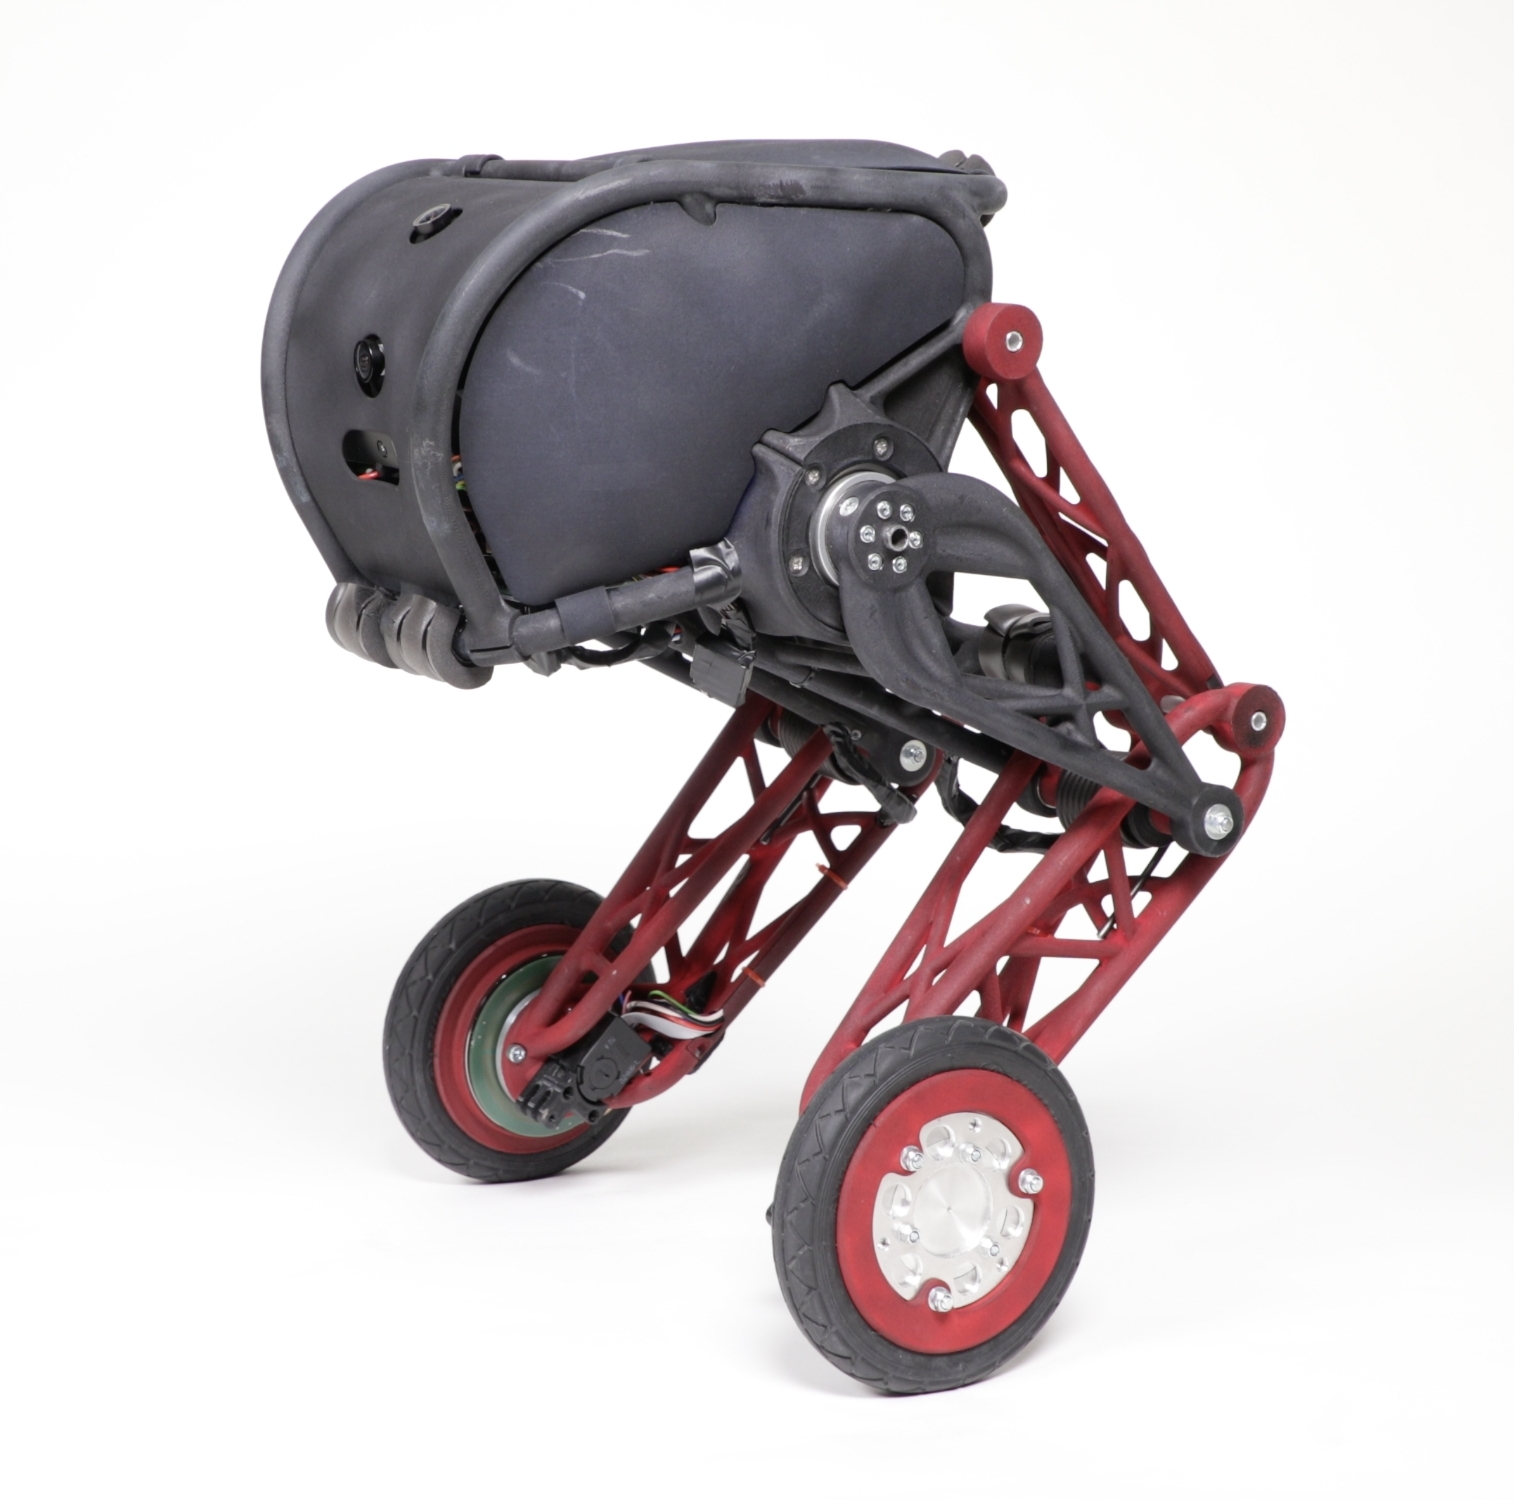
\includegraphics[width=0.5\textwidth]{Ascento robot}
\caption{Ascento Robot by ETH Zurich\cite{klemm2019ascento}}
\label{fig:Ascento robot}
\end {figure}

The Legged Two-Wheeled Inverted Pendulum Robot (LTWIPR) is a type of mobile robot that has two wheels and a body carried by two legs.
The robot acts as an inverted pendulum, with the wheels acting as the pivot point.
The robot is able to balance itself on the two wheels. The robot is able to move by tilting the body forward or backward, causing the wheels to rotate in the direction of the tilt. The robot is able to turn by moving the wheels in opposite directions. The robot is able to move in any direction by combining these movements. LTWIPRs are able to move in a variety of environments, including rough terrain and stairs. LTWIPRs are able to perform complex movements, such as jumping and climbing. LTWIPRs are able to interact with their environment, such as navigating around obstacles and diving under obstacles.



\section{Prior Works and Advances in Multi-Legged Robotic Systems}
%This section should provide a comprehensive review of existing literature relevant to your research topic. It should cover key theories, models, experiments, and findings in the field, particularly focusing on works that directly relate to your research question or hypothesis. This review not only shows your understanding of the field but also how your work fits into and contributes to the existing body of knowledge.
\subsection{Mechanical Design and Development of Wheeled Robots}

\subsection{Dynamic Modeling of Wheeled Bipedal Robots}
\subsection{Control of Wheeled Bipedal Robots}
\subsection{Integration of Learning and Adaptive Control Mechanisms in Wheeled Bipedal Robots}
\subsection{Applications and Future Directions}

